\subsection{Questions}
\begin{enumerate}
	\item In this experiment, What parameter do we measure?
	\begin{itemize}[label=-]
		\item The peak height of the bank: Standard $Z$.
		\item Water level $Z$ in the canal at each flow rate mode.
		\item The time to calculate the flow rate.
	\end{itemize}
	\item While conducting the experiment, which tools do we need? What are they use for?
	\begin{itemize}[label=-]
		\item Hydraulic table consists of rectangular overflow bank mounted on the canal: to change the mode of water flow through the overflow bank.
		\item Stopwatch: determine the time to calculate the flow rate.
		\item Balance ruler: measure the peak height of the bank.
	\end{itemize}
	\item Before checking the water level $Z$, what we need to do?
	\begin{itemize}[label=-]
		\item Check the stability of water level.
		\item Check and adjust the valve so that the water level rises and encounters the head of needle.
	\end{itemize}
	\item What is the function of wave screen in this experiment?\\
	The wave screen is used  to minimize the fluctuation of the water level due to the wave.
	\item How many flow rate mode should we conduct? How many times does each flow rate mode need to be repeated?\\
	We conduct at 4 flow rate mode and each mode repeat 3 times
\end{enumerate}
\subsection{Measurements}
Water temperature: $t \degree = 35 \degree C$
{
\newcolumntype{L}[1]{>{\raggedright\let\newline\\\arraybackslash\hspace{0pt}}m{#1}}
\newcolumntype{C}[1]{>{\centering\let\newline\\\arraybackslash\hspace{0pt}}m{#1}}
\setlength{\parskip}{1em}
\setlength{\parindent}{0in}
\renewcommand*\arraystretch{1.5}

\begin{table}[ht]
	\centering
	\hspace*{-1cm}
	\begin{tabular}{cllllccccccc}
		\toprule
		\multirow{3}{*}{No.} & \multicolumn{3}{c}{Raw data}                                                     & \multicolumn{8}{c}{Calculated data}                                                                                                                                                                                                     \\ [0.5ex] \cmidrule{2-5} \cmidrule{6-12}
		& $Z_i$   & $\Delta V$ & $\ Del t$  &$Q_i$   & $Z_{avg}$              & $H$                   & $Q_{avg}$                 & \multirow{2}{*}{$\log H$} & \multirow{2}{*}{$\log Q$} & \multirow{2}{*}{$C_d$ experiment} & \multirow{2}{*}{$C_d$ Tsugaev} \\
		& \multicolumn{1}{c}{($cm$)} & \multicolumn{1}{c}{($l$)} & \multicolumn{1}{c}{($s$)} & \multicolumn{1}{c}{($\frac{l}{s}$)} & ($cm$)                   & ($cm$)                  & ($\frac{cm^3}{s}$)                &                           &                           &                                     &                                \\ \hline
		\multirow{3}{*}{1}   & 13.14                    & 5                           & 16.7                    & 0.3                           & \multirow{3}{*}{13.13} & \multirow{3}{*}{1.16} & \multirow{3}{*}{301.41} & \multirow{3}{*}{0.06}     & \multirow{3}{*}{2.48}     & \multirow{3}{*}{0.809}              & \multirow{3}{*}{0.612}         \\
		& 13.13                    & 5                           & 16.4                    & 0.3                           &                        &                       &                         &                           &                           &                                     &                                \\
		& 13.13                    & 5                           & 16.7                    & 0.3                           &                        &                       &                         &                           &                           &                                     &                                \\ \hline
		\multirow{3}{*}{2}   & 12.73                    & 5                           & 12.44                   & 0.4                           & \multirow{3}{*}{12.73} & \multirow{3}{*}{1.56} & \multirow{3}{*}{403.56} & \multirow{3}{*}{0.19}     & \multirow{3}{*}{2.61}     & \multirow{3}{*}{0.694}              & \multirow{3}{*}{0.615}         \\
		& 12.73                    & 5                           & 12.42                   & 0.4                           &                        &                       &                         &                           &                           &                                     &                                \\
		& 12.74                    & 5                           & 12.31                   & 0.41                          &                        &                       &                         &                           &                           &                                     &                                \\ \hline
		\multirow{3}{*}{3}   & 12.35                    & 5                           & 8.74                    & 0.57                          & \multirow{3}{*}{12.34} & \multirow{3}{*}{1.95} & \multirow{3}{*}{570.14} & \multirow{3}{*}{0.29}     & \multirow{3}{*}{2.76}     & \multirow{3}{*}{0.702}              & \multirow{3}{*}{0.619}         \\
		& 12.34                    & 5                           & 8.74                    & 0.57                          &                        &                       &                         &                           &                           &                                     &                                \\
		& 12.34                    & 5                           & 8.83                    & 0.57                          &                        &                       &                         &                           &                           &                                     &                                \\ \hline
		\multirow{3}{*}{4}   & 11.94                    & 5                           & 6.63                    & 0.75                          & \multirow{3}{*}{11.93} & \multirow{3}{*}{2.36} & \multirow{3}{*}{757.59} & \multirow{3}{*}{0.37}     & \multirow{3}{*}{2.88}     & \multirow{3}{*}{0.7}                & \multirow{3}{*}{0.622}         \\
		& 11.93                    & 5                           & 6.57                    & 0.76                          &                        &                       &                         &                           &                           &                                     &                                \\
		& 11.91                    & 5                           & 6.6                     & 0.76                          &                        &                       &                         &                           &                           &                                     &                                \\ \bottomrule
	\end{tabular}
	\hspace{-2cm}
	\caption{Rectangular weir, $Z_{std}=14.29cm$}
\end{table}}

\subsection{Calculations and Report}
\begin{enumerate}[label=\textbf{\Alph*.}]
	\item Calculations:
	\begin{enumerate}
		\item Calculate the flowrate $Q_i$ in each test and the average value $Q_{avg}$ of each test.
		\item Calculate $Z_{avg}$ of each test and the height of water $H$ on the top of the weir.
	\end{enumerate}
	\item Determine the coefficient flowrate $C_d$ of the rectangular weir.
	\begin{enumerate}
		\item Calculate Cd, assuming the coefficient is constant.
		\begin{itemize}[label=-]
			\item Calculate $\log Q$, $\log H$ for each test.
			\item Draw a relation graph $\log Q = f(\log H)$ on Fig \ref{fig1lab6}.
		\end{itemize}
		\item Determine the intersection between the graph and its vertical axis, $b$ and the coefficient of flow rate $C_d$.\\
		$b=2.37$\\$C_{d(rec)}=0.786$
		\item Determine the coefficient of flow rate $C_d$ by formula (6.16) for each test. Draw the relation graph $C_d=f(H)$.
		\item Determine the coefficient of flow rate by Tsugaev formula for each test. Draw the relation graph $C_d=f(H)$.
	\end{enumerate}
	\item Conclusion
	\begin{enumerate}
		\item On Figure \ref{fig1lab6}, is the relation graph $\log Q = f(\log H)$ linear according to the plotted data? If not, explain (e.g. measurement errors).
		\begin{figure}[H]
			\centering
			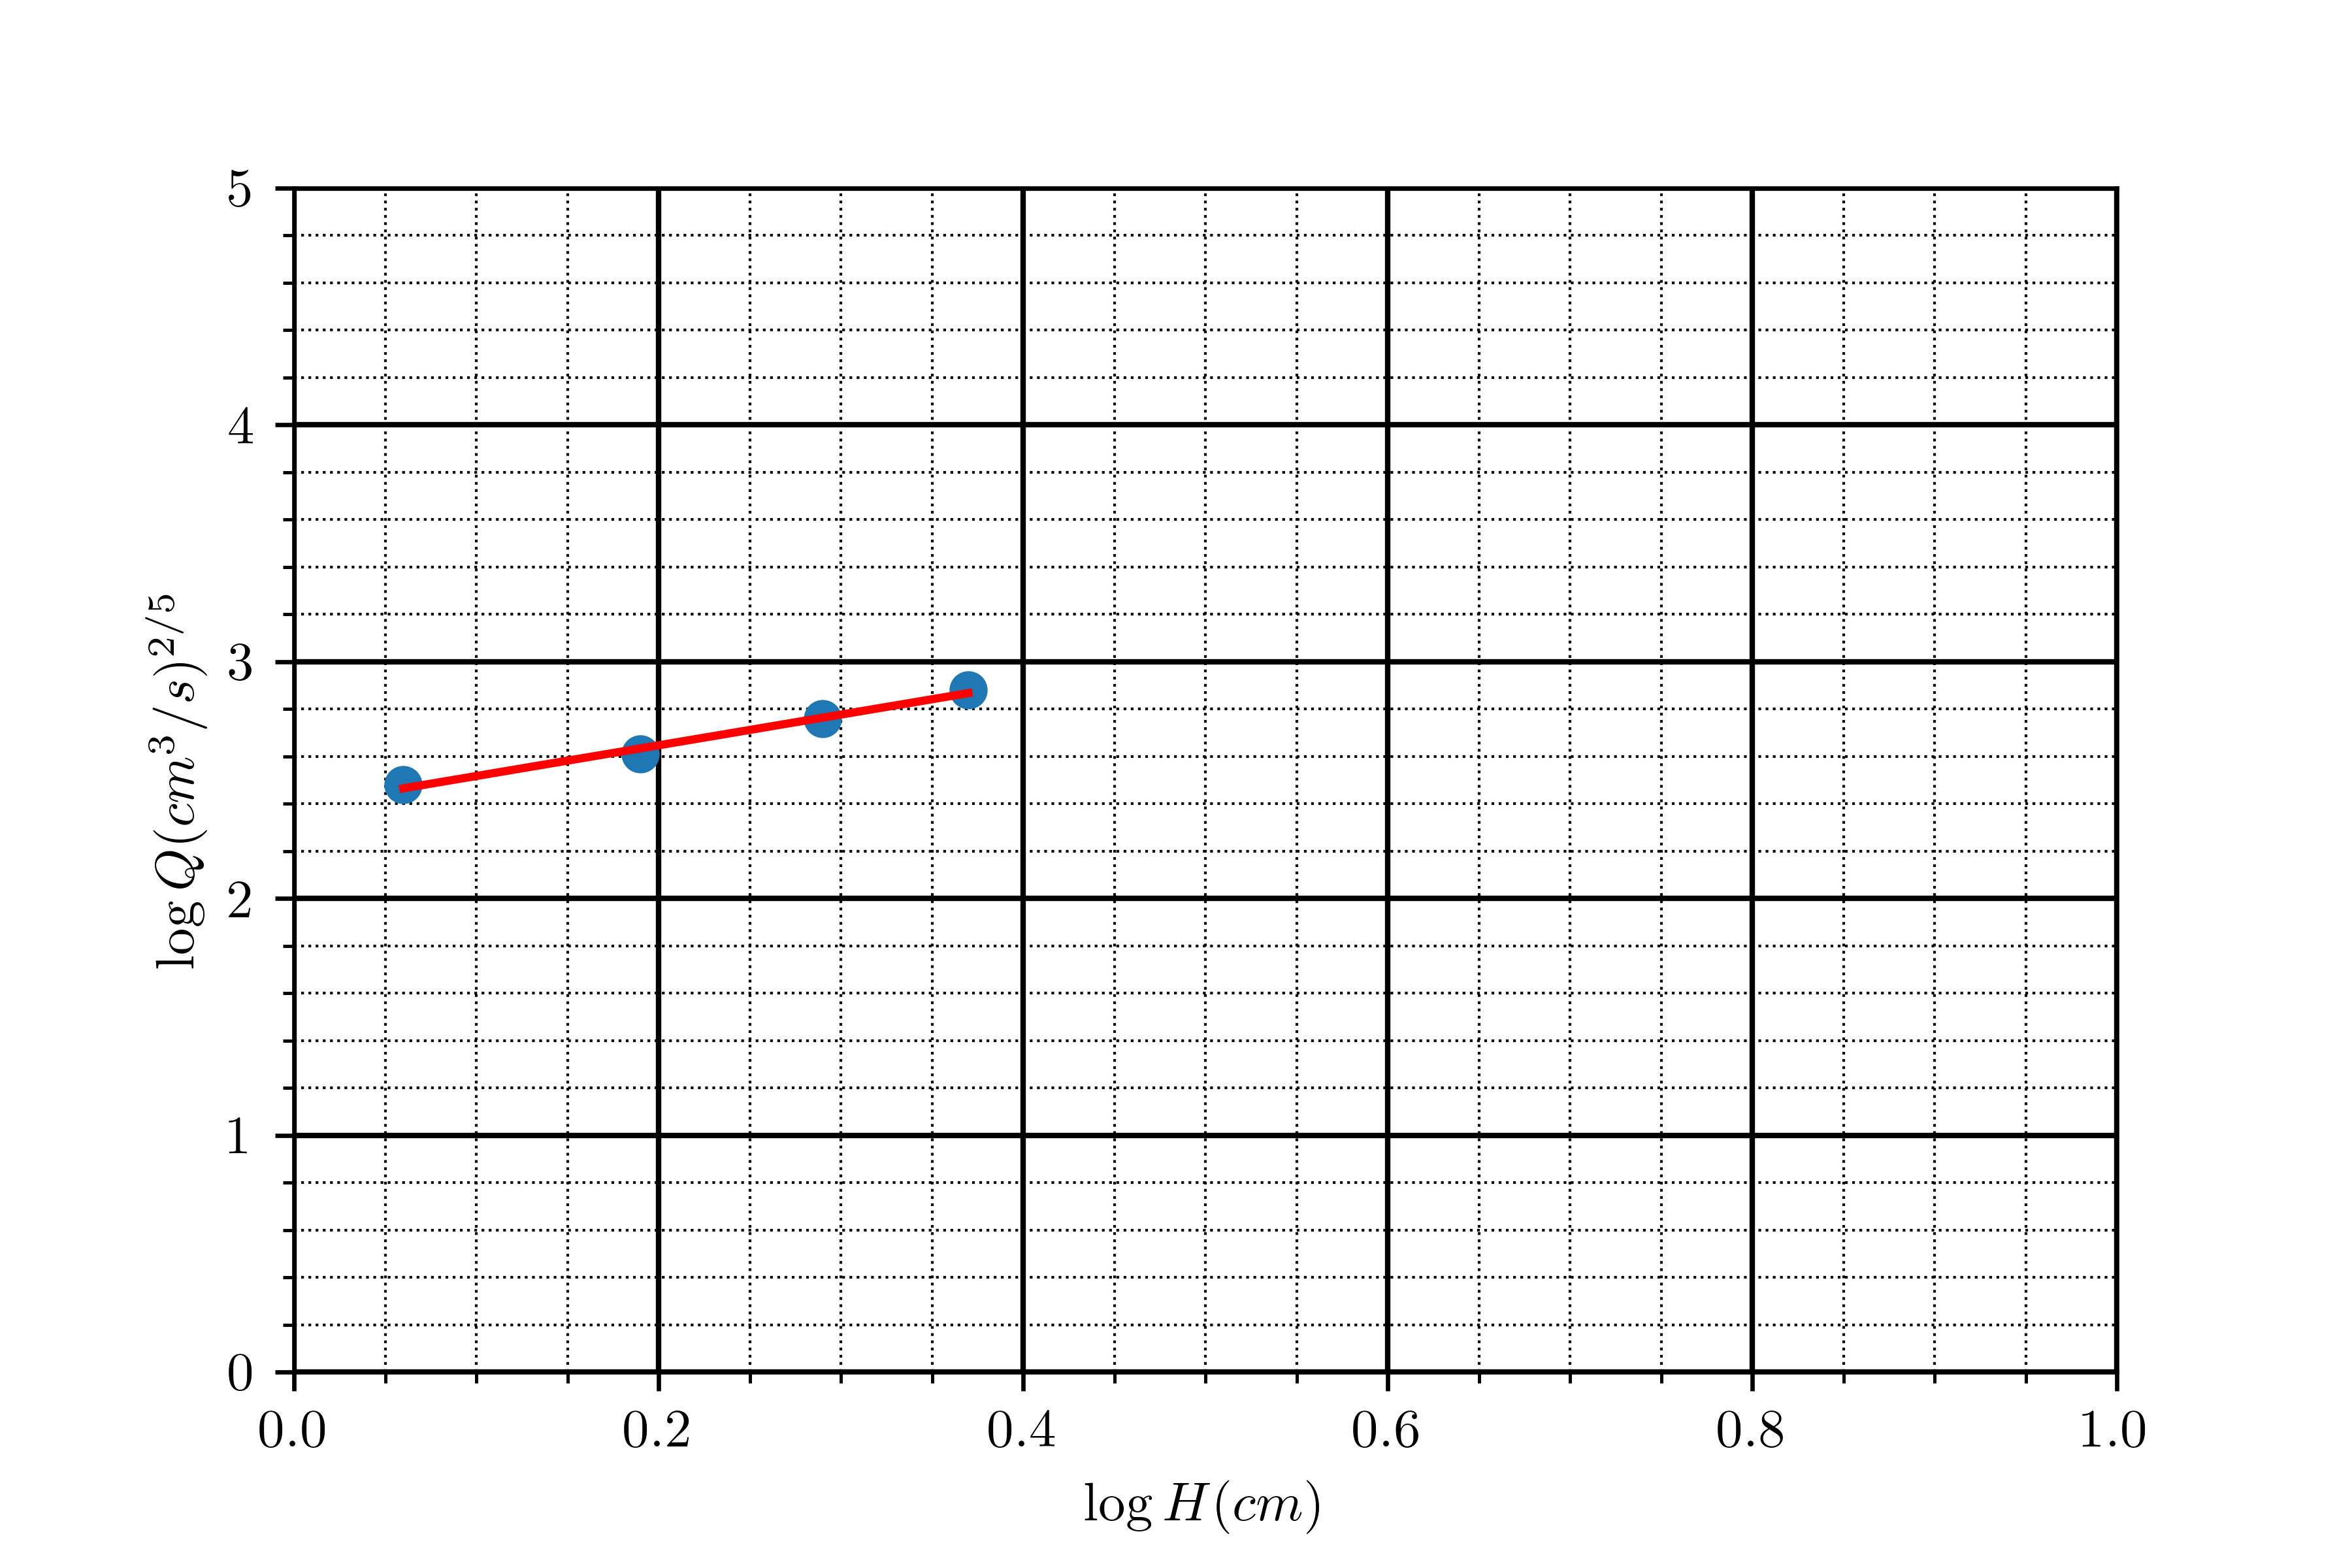
\includegraphics[width=150mm]{photos/fig1lab6.png}
			\caption{Relation graph $\log Q = f(\log H)$ of the rectangular weir}
			\label{fig1lab6}
		\end{figure}
		\item What is the shape of the relation graph $C_d=f(H)$? Explain.
		\begin{itemize}[label=-]
			\item The relation graph $C_d=f(H)$ is not linear.
			\item Explain:
			\begin{itemize}[label=+]
				\item Errors when students measure data.
				\item Instrumental error (Stop-watch, ruler, …).
				\item Loss of energy.
			\end{itemize}
		\end{itemize}
		\begin{figure}[H]
			\centering
			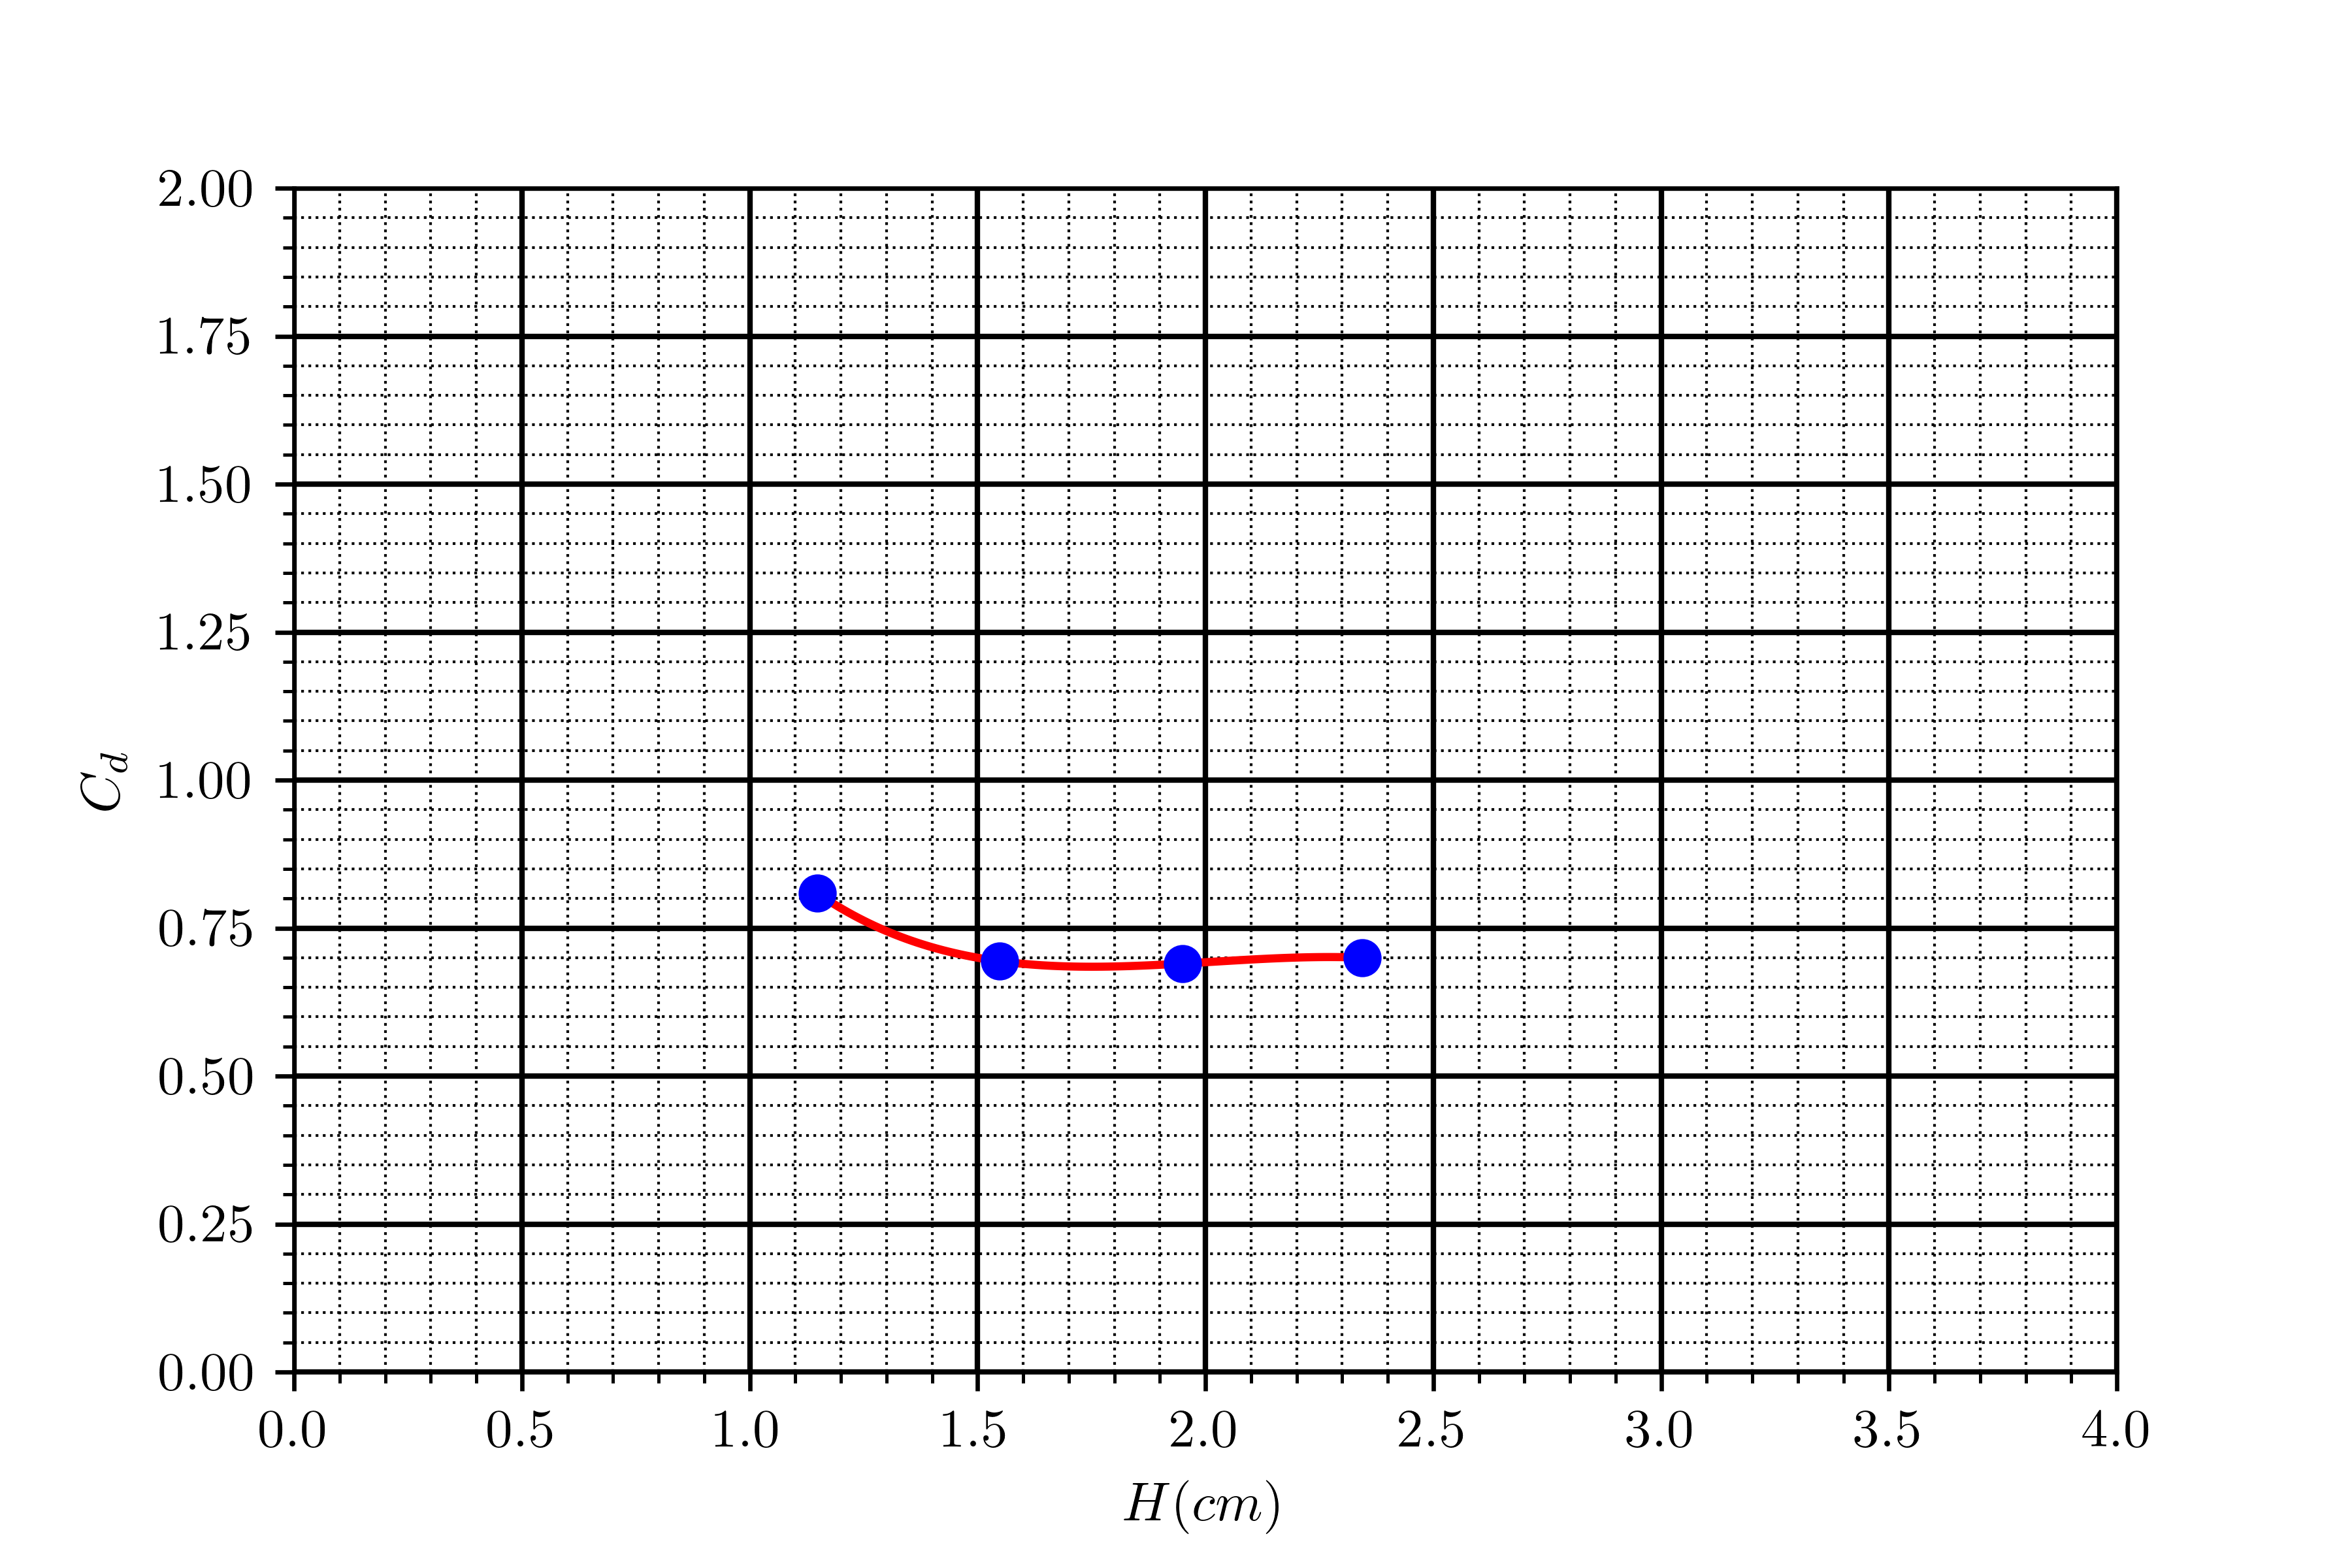
\includegraphics[width=150mm]{photos/fig2lab6.png}
			\caption{Relation graph $C_d=f(H)$ of the rectangular weir}
			\label{fig2lab6}
		\end{figure}
	\item Compare the value result from the experiment and from the Tsugaev formula. If it has different, state the reason.
	\begin{itemize}[label=-]
		\item The value $C_d$ from the experiment and from the Tsugaev formula has different result.
		\item Explain:
		\begin{itemize}[label=+]
			\item Error when measuring the water level of the weir.
			\item Measure the water level of the weir when the water surface is no stable.
			\item Instrumental error (Stop-watch, fluid tank, …)
		\end{itemize}
	\end{itemize}
	\end{enumerate}
\end{enumerate}
